%%%%%%%%%%%%%%%%%%%%%%% file template.tex %%%%%%%%%%%%%%%%%%%%%%%%%
%
% This is a general template file for the LaTeX package SVJour3
% for Springer journals.          Springer Heidelberg 2010/09/16
%
% Copy it to a new file with a new name and use it as the basis
% for your article. Delete % signs as needed.
%
% This template includes a few options for different layouts and
% content for various journals. Please consult a previous issue of
% your journal as needed.
%
%%%%%%%%%%%%%%%%%%%%%%%%%%%%%%%%%%%%%%%%%%%%%%%%%%%%%%%%%%%%%%%%%%%


\RequirePackage{fix-cm}
%
%\documentclass{svjour3}                     % onecolumn (standard format)
%\documentclass[smallcondensed]{svjour3}     % onecolumn (ditto)
%
%\documentclass[smallextended]{svjour3}       % onecolumn (second format)
\documentclass[twocolumn]{svjour3}          % twocolumn
%
\smartqed  % flush right qed marks, e.g. at end of proof
%
\usepackage{graphicx}
\usepackage[spanish]{babel}
% \usepackage{mathptmx}      % use Times fonts if available on your TeX system
%
% insert here the call for the packages your document requires
%\usepackage{latexsym}
% etc.
%
% please place your own definitions here and don't use \def but
% \newcommand{}{}
%
% Insert the name of "your journal" with
\journalname{Autonomous Robots}
%
\begin{document}

\title{Jderobot open source framework for robotic, computer vision and home automation applications
%\thanks{Grants or other notes
%about the article that should go on the front page should be
%placed here. General acknowledgments should be placed at the end of the article.}
}
%\subtitle{Do you have a subtitle?\\ If so, write it here}

%\titlerunning{Short form of title}        % if too long for running head

\author{Jos\'e M. Ca\~nas \and David Lobato \and Roberto Calvo \and Julio Vega \and Eduardo Perdices \and Francisco Rivas}

%\authorrunning{Short form of author list} % if too long for running head

\institute{F. Author \at
              first address \\
              Tel.: +123-45-678910\\
              Fax: +123-45-678910\\
              \email{fauthor@example.com}           %  \\
%             \emph{Present address:} of F. Author  %  if needed
           \and
           S. Author \at
              second address
}

\date{Received: date / Accepted: date}
% The correct dates will be entered by the editor


\maketitle

\begin{abstract}
For a given robot most of its intelligence lies on its software, the way it coordinates its sensing and actuation capabilities. In the last years several frameworks have appeared that simplify and speed up the development of robot applications. They favor the code reuse and take benefits from modern software engineering techniques. This paper presents the open source robotics framework Jderobot, a distributed and component oriented platform. It uses explicit interfaces among components and ICE as communication middleware. It provides many tools for robot programming like a template for robot control components, visual HFSM creation, etc. Several examples of research and applications done with this framework are also described as experimental validation of it.
\keywords{Robot software \and Programming frameworks \and Code reuse}
% \PACS{PACS code1 \and PACS code2 \and more}
% \subclass{MSC code1 \and MSC code2 \and more}
\end{abstract}

\section{Introduction}
\label{intro}

%software importance
Most of robot intelligence lies on its software. Once the robot sensor and actuator devices are set, the robot behavior is fully caused by its software. There is no universally accepted way of programming robots. There are robots programmed in low level assembler and also in high level languages like C, C++ or Java. 

The importance of good programming practices has increased in the last years and also the interest in the robotics community on this topic. Several special issues of robotics journals (ARS Special Issue on Software Development and Integration in Robotics, 2006) and books on the topic \cite{brugali2007} have been published, specific workshops have been created inside ICRA and IROS, the Journal of Software Engineering for Robotics (www.joser.org) has appeared that promotes the synergy between Software Engineering and Robotics, and the Technical Committee for Software Engineering for Robotics and Automation inside the IEEE Robotics and Automation Society (TC-SOFT) has been created. Code reuse to avoid restarting from scratch for every new robot platforms and software integration are key issues in this topic. 

%Encapsulating robot capabilities in functions is a slippery issue as behaviors usually don't fit into the functional abstraction where the caller invokes the function and stops it flow of execution until receives the function response or output.

% software requirements in robotics
Compared with other computer science fields the development of robot applications exhibits some specific requirements. First, liveliness and real-time processing: software here has to take decisions with in a fast way, for instance in robot navigation or image processing. Second, robot software has to deal with multiple concurrent sources of activity, and so tends to be multitask. Third, computing power is usually spread along several connected computers, and so the robotic software may be distributed. Fourth, the robotic software typically deals with heterogeneous hardware. New sensor and actuator devices continually appears in the market and this makes maintenance and portability to new robots or devices more complex. Fifth, the robotic software usually includes a Graphical User Interface, mainly for debugging purposes. Sixth, the robotic software should be expansible for incremental addition of new functionality and code reuse. Seventh, the simulators are very useful in robotics software debugging.

% robotic frameworks 
Mobile robot programming has evolved significantly in recent years, and two approaches are currently found. In the classical approch the application programs for simple robots obtain readings from sensors and send commands to actuators by directly calling functions from the drivers provided by the seller. In last years several frameworks (SDKs) have appeared that simplify and speed up the development of robot applications, both from robotic companies and from research centers, both with closed and open source. They favor the portability of applications between different robots and promote code reuse.

First, they offer a simple and more abstract access to sensors and actuators than the operating systems of simple robots. Using the SDK hardware abstraction layer it deals with low level details accessing to sensors and actuators, releasing the robotics programmer from that complexity.
%For example, in a Pioneer with a laser rangefinder, the applications can obtain readings using ARIA or directly through a serial port. Using ARIA, one need only invoke a method and ARIA will take charge of refreshing the variables. Using the operating system directly, the application must request and periodically read the data from the laser through the serial port, and must identify the protocol of the device to compose and analyze the low level messages correctly. The abstract access is also offered for actuators.

Second, the SDK provides a software architecture for robot applications. It offers a particular way to organize code, allowing the handling of code complexity when the robot functionality increases. There are many options: calling to library functions, reading variables, invoking object methods, sending messages via the network to servers, etc.. Depending on the programming model the robot application can be considered an object collection, a set of modules talking through the network, an iterative process calling to functions, etc.

Third, usually the SDK includes simple libraries, tools and common use functionality blocks, such as robust techniques for perception or control, localization, safe local navigation, global navigation, social abilities, map construction, etc. This way SDKs shorten the development time and reduce the programming effort needed to code a robotic application as long as the programmer can build it by reusing the common functionality included in the SDK, keeping herself focused in the specific aspects of her application. The robot manufacturers sell them separately or include them as additional value with their own SDKs. For example, ERSP includes three packages in the basic architecture: one for interaction, one for navigation and another for vision. 

% our proposal
We present our open-source robotic software framework, named Jderobot, which is component oriented, uses ICE as communication middleware and includes several useful tools and libraries. Several sensor and actuator drivers have been programmed or reused from the open-source community. This framework has been widely used in our group for research and teaching for more than ten years. Jderobot has been designed for scenarios with sensors, actuators and intelligent software in between. The typical scenario is robotics, but also computer vision and home automation.

% open source
Why open-source in robotics? First, it provides independence on robot manufacturers and so it may support robots from different companies. Using open-source you are free to modify, debug, or improve the software, so the final software quality is high and does not depend on a single company debuggins speed. One strong motivation is also the feeling of contributing to the robotics community and to return the favor. We have extensively used open-source libraries and tools in our research (OpenCV, Gazebo, GTK, etc.). Research algorithms can be replicated easily and compared with standard tools. The tools must be open in order to trust in them.

% paper organization
This paper is organized as follows. The state of the art in robotic frameworks fills section \ref{sec:relatedworks}, where other platforms are briefly presented. Section \ref{sec:jderobot} fully explains the proposed platform, the ideas behind its design, the set of standardized interfaces and developed drivers, and the tools included to make the development of new applications easier. In section \ref{sec:applications} some successful examples using Jderobot are presented, both in research and in teaching. Final section summarizes the main conclusions and lessons learnt.

\section{Related works}
\label{sec:relatedworks}

Robotic frameworks can be grouped in two main paradigms, those tightly
coupled with a cognitive model in their designs and those designed
just from a pure engineering criteria. The first ones \textit{force}
the user to follow a set of rules in order to program certain robotic
behavior, while the second ones are just a collection of tools that
can flexibly be put together in several ways to accomplish the task.

%cognitive frameworks
Cognitive robotic frameworks were popular in the 90s and they were
strongly influenced by the AI, where planning was one of the main
keys. Indeed one of the strengths of such frameworks were their
planning modules built around a sensed reality. A good example of cognitive
frameworks was Saphira \cite{konolige98} based on a behaviourist
cognitive model. Some of its low-level functionality was rewritten as a
C++ library called ARIA \cite{aria} that it's still supplied with the
popular robotic platforms from MobileRobots/ActivMedia.

%current frameworks
Current robotic frameworks focus their designs on the requirements
that robotics applications need and let the user (the programmer) to
choose the organization that better fits with her specific
application. Main requirements driving the designs are: multi-tasking, distributed, easy to
use and code reusability. Another requirement, we believe it's a main
key, it's the open source code, that creates a synergy between the use
and the developer. Proof of this is the two most popular robotic
frameworks in the last years: PlayerStage
\cite{Gerkey03,collet05,vaughan2007} which has been the \textit{standard de
facto} in most of the last decade and ROS \cite{quigley09} which is
taking the place currently.

%key achievements
Key achievements of modern frameworks are the hardware abstraction, hiding the complexity of accessing heterogeneous hardware (sensors and
actuators) under standard interfaces, the distributed capabilities
that allows to run complex systems spread over a network of computers,
the multi-platform and multi-language capabilities that enables the
user to run her software in multiple architectures, and the existence
of big communities of software that share code and ideas.

%examples
Main examples of modern frameworks are the aforementioned PlayerStage
and ROS. The first has two main parts, Player, provides a network
interface to the robot hardware through a collection of standard
interfaces. This standard interfaces are implemented by drivers, one
for each different hardware. This way a user only needs to know the
standard way to use, let say, a laser ranger and not every different
brand. The second part is Stage, a 2D simulator that allows the user
to try in a simulated world before trying on a real platform. In
addition to this, PlayeStage framework provides a variety of
algorithms that are used with the same concept through standard
interfaces. Other example is ROS that employs the same concept of
standard interfaces with the addition of a middleware that greatly
simplifies the network distribution. The core system of ROS comes with
a collection of tools to help with tasks as project management, system
debugging and centralized logging. Currently has a growing community
and its site hosts a great collection of hardware drivers, algorithms
and other tools.

Another important example is ORCA \cite{brooks05,brooks07} based on the
same concepts mentioned, but with the idea of expending less effort
building the underlying middleware elements . This way they chose to
use Ice from ZeroC \cite{henning04}, a powerful object oriented middleware
that allows them to focus in the robotic problems.

%%CARMEN \cite{montemerlo03}
%%ROS, ORCA, Miro, RoboComp, Aria, 
%%Microsoft Robotics Studio, Beesoft. ERSP.

\section{Jderobot platform}
\label{sec:jderobot}

Some history. Keep away the cognitive ideas, focus on software
architecture. Nace como implementación de arquitectura cognitiva,
tesis doctoral jdec \cite{canas02}. Evolucionó a una plataforma de programación para
aplicaciones robóticas, domóticas y de visión computacional (sensores,
actuadores, inteligencia).



\begin{itemize}
\item Orientada a componentes distribuidos y multilenguaje
\item La mantiene un grupo de desarrolladores, es abierta
\item {http://jderobot.org}, manuales, descarga, ejemplos
\end{itemize}
Software libre (licencia GPLv3), paquete debian


Arquitectura cognitiva JDE:
\begin{itemize}
\item Comportamiento = {percepción} y {control}
\item Fragmentación en unidades asíncronas concurrentes (esquemas)
\begin{itemize}
\item[-] de percepción elaboran estímulos
\item[-] de actuación toman decisiones
\end{itemize}
\item La colección de esquemas se organiza en \textit{jerarquía} dinámica (JDE)
\item Sigue el paradigma basado en comportamientos
\end{itemize}

Arquitectura cognitiva: Esquemas.
Un {esquema} es un flujo de ejecución independiente, con un objetivo
\begin{itemize}
\item Funcionamiento continuo
\item Se puede activar y desactivar a voluntad
\item Modulable a través de parámetros
\item Su funcionalidad se usa despertándolo y modulándolo
\item {Perceptivos}: producen estímulos (piezas de información) y los mantienen actualizados. Lecturas sensoriales, transformaciones más elaboradas 
\item {Actuación}: toman decisiones para conseguir o mantener un objetivo, comandos a los actuadores o la activación y modulación de otros 
\end{itemize}



\subsection{Software architecture design}

Some history and lessons learnt: 4.3. 

Threads. GUI specific interface. 

\begin{itemize}
\item Component oriented 
\item Iterative execution
\item Concurrent and optional visualization
\item Processes better than threads
\item ICE for communication
\item Explicit standard interfaces
\item Configuration files 
\end{itemize}

multilanguage, distributed intermachine, Android, efficient

Reuse other open-source libraries: OpenCV, Gearbox, GTK, PCL, OpenGL, PlayerStage, Gazebo, GSL, Cwii.


GUI thread separated from control thread.
Iterative control, iterative perception. Component frequency.
Standard interfaces for communication with other components.

Modelo de programación: Componente
\begin{itemize}
\item Cada esquema se materializa en un {componente} software 
\item El funcionamiento continuo como {ejecución iterativa}, iteraciones periódicas a cierto ritmo para percibir o para actuar
\item Ofrece funcionalidad y usa la de otros a través de {interfaces} explícitos
%el componente es la unidad básica
\item Aplicación $=$ conjunto de componentes concurrentes que interoperan
\item {Multimáquina} y {multilenguaje}: C, C++, python, Java... 
\item Usa el middleware de comunicaciones ICE (zeroC)
\end{itemize}

Ejecución iterativa:
\begin{itemize}
\item Iteración de control o de percepción
\item component\_cycle 
\item \texttt{gettimeofday}
\item \texttt{usleep}
\item Espera condicional
\item Patrón de diseño \textit{Algoritmo iterativo}
\end{itemize}

Interfaces tipados
\begin{itemize}
\item {Comunicación entre componentes}, conexión con otros 
\item Fijan la estructura de los datos que el componente ofrece o necesita
%\item Invocar funciones del interfaz
\item Cada componente puede necesitar y ofrecer uno o varios interfaces 
%espacio de nombres
\item Se definen con \texttt{slice}
\item Generación de código para múltiples lenguajes (C++, Java, Python...)
\item Mecanismos de transmisión de datos eficientes
\begin{itemize}
\item transmisión síncrona o asíncrona
\item publicación/subscripción
\end{itemize}
\end{itemize}


Visualización
\begin{itemize}
\item {Modular} y {opcional}: cada componente tiene (o no) su propio GUI
\item Cada componente incluye el código de su interfaz gráfica
%\item Activable/desactivable a voluntad, cuando interesa
\item Mostrar e interacción con humano 
\item Depuración, útil en desarrollo
\item GTK, XForms, OpenGL
\item Patrón de diseño \textit{Modelo Vista Controlador}
\item Se materializa en una {hebra adicional}
\end{itemize}



Ficheros de configuración:
\begin{itemize}
\item Cada componente puede tener el suyo 
\item Ficheros de configuración ICE
\item Especifican cuál es la fuente de cada interfaz (local o remota)
\item Parámetros específicos
\end{itemize}

\subsection{Interfaces and drivers}


Acceso a los dispositivos hardware
\begin{itemize}
\item Se da a través de {componentes drivers}
\item Acceden localmente al sensor/actuador y ofrecen acceso (local o remoto) a otros a través de interfaces ICE
\item No suelen tener GUI
\item El mismo interfaz de datos lo puede proporcionar varios \textit{drivers}
\begin{itemize}
\item Mismo programa funciona sobre robot real o simulador
\item Independencia de la fuente de imágenes
\end{itemize}
\end{itemize}


Standard interfaces. 
PlayerServer, GazeboServer for Gazebo Simulator , NaoServer, KinectServer, OpenNIServer, giraffeServer, PTU, Hokuyo, Wiimote, CameraServer.

Same interfaces for different robots.
Applications run exactly the same on real robot than on simulator. 

\subsubsection{PlayerServer and GazeboServer}
\label{subsec:gazeboserver}

Jderobot integrates two servers, named PlayerServer and GazeboServer, which are used to communicate Player and Gazebo simulators (\cite{koening2004}) with other software components in the Jderobot platform. It's possible to retrieve information from several sensor devices, such us: laser, encoders, motors, cameras or sonars. And it also supports one or more cameras with their pantilt units (SonyVid30 model).

\subsubsection{NaoServer}

Nao robots include an internal Framework called ''Naoqi'', which provides an API to command and read the robot's motors and sensors. This API can't be directly deployed by other Jderobot components, since its functions are ad-hoc designed to Nao robots.

We have created an application called NaoServer, that runs inside the Nao robots and provides several standard ICE interfaces which may be used by other Jderobot components. NaoServer receives through ICE interfaces commands from other components and translates these commands to Naoqi.

\subsection{Tools and libraries}

\subsubsection{FuzzyLib}: control borroso
\subsubsection{VisionLib}
\label{subsec:visionlib}

Mathematical functions used on visual perception purposes can be found on this vision library. It contains computer vision research code initially developed to support the RobotVision project. It has since been expanded to provide a range of software infrastructure for computer vision, geometry models and images mechanisms. The library builds on top of the OpenCV Computer Vision Library\footnote{http://opencv.willowgarage.com/wiki} and the GNU Scientific Library\footnote{http://www.gnu.org/software/gsl} (GSL).

The structure of this library is as follows:
\begin{itemize} 
\item \textit{Cvfast} class provides the functionality of the Image Corner Detector called FAST.
\item \textit{Geometry} class contains implementations of different visual geometry purposes: intersections, distances, vector operations, segments operations, etcetera.
\item \textit{Image} class includes operations such as: Multiply Fast Fourier Transform or Get Segments.
\item \textit{LinesDetection} class provides the implementation of an Image Border Detector based on an article by A. Solis (\cite{solis09}).
\item \textit{Structs.h} header contains different useful structs for computer vision purposes.
\end{itemize}

\subsubsection{Progeo}
\label{subsec:progeo}

In order to facilitate the use of pin-hole calibrated cameras (see Figure \ref{fig:pinholemodel}) as well as certain geometry functions used for the purposes of performing 2D and 3D images calculations (such as 2D to 3D transformation and viceversa), Jderobot provides a library called ProGeo.

\begin{figure}[h!]
  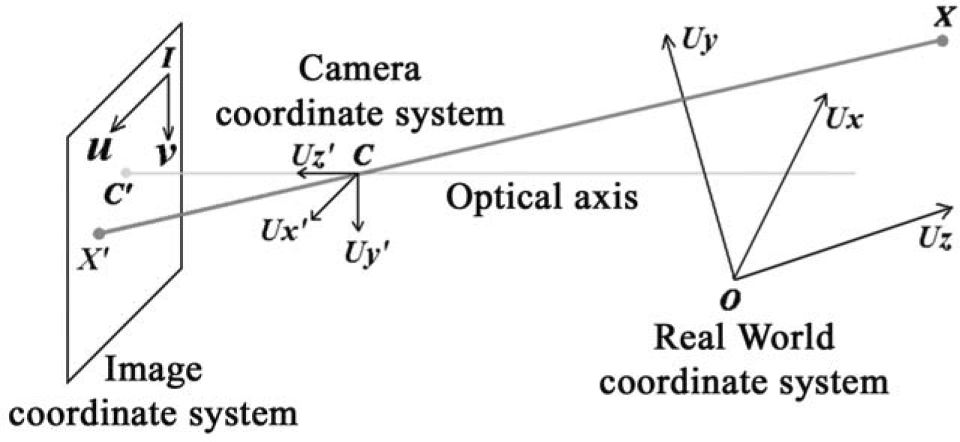
\includegraphics[width=8.5cm]{figs/pinholemodel.png}
\caption{Pin-hole model of a camera.}
\label{fig:pinholemodel}
\end{figure}

Some of the data types provided by this library are: \textit{HPoint2D} (to store a 2D point that usually belongs to the image plane), \textit{HPoint3D} (data point structure that represents a point in the 3D space) or \textit{TPinholeCamera} (pin-hole camera model defined by its extrinsics and intrinsics parameters).

And some of the functions which can be found are: \textit{project} (to project a 3D point on to the 2D image planer) and \textit{backproject} (to obtain the projection line that connects the camera with the focus and the 3D ray which is projected in a pixel of the image plane).

\subsubsection{Colorspaces}: espacios de color para imágenes

\subsubsection{Control template}
Basic component for reactive controllers



\subsubsection{VisualHFSM}
\subsubsection{Calibrator}
\subsubsection{ColorTuner}
\subsubsection{Recorder and replayer}

When we use real robots, one of the greatest difficulties is repeating experiments with the same conditions, whether we want to compare different algorithms or to test several features of the same algorithm. It's almost impossible to reproduce the same environment conditions, since robot hardware behaves diversely, light conditions change if we use cameras, people or objects move or are located in different places, etc.

To avoid all these matters, we have designed a new tool which records the current devices status and reproduces them whenever we want to. There are two components involved in this tool, the first one is the so-called ''recorder'', it saves in a file the status of all the devices of the robot, such as odometry, laser measures, image cameras, etc; we can configure which devices we want to track when we executes the components and it works with simulators, real Nao robots and real Pioneer robots.

The second components is the ''replayer'' component, it reads the file saved by the ''recorder'' component and provides the same ICE interfaces that would provide the real devices. Thus, when an algorithm gets the current devices status, it can't tell if it's obtaining the current devices measures in real time or pre-recorded data.

This tools has been widely used to perform experiments with real robots, to try different parameters and improve our algorithms.

\subsubsection{Android mobileTeleoperator}

Android operating system is increasing its market share every day, both with smartphones and tables. Once you develop an application for this platform, it may be used by students, other researchers or even companies. 

We have created an application called ''Mobile Teleoperator'' to teleoperate either a Pioneer robot with playerserver or a Nao Robot with BICA architecture. Connection among the mobile device and the robots is made through ICE, the same way we do when we use a standard computer, so we don't need to change anything in Jderobot architecture.

There are three ways to teleoperate the robots:
- Arrows: After pressing a button, it sends the command to the robot and the robot keeps his behavior until the stop button is pressed.
- Joystick: While a button is pressed, it send the command to the robot, but if the button is released it sends a stop command automatically.
- Accelerometer: It uses the mobile accelerometers to command the robot depending on our device orientation. To use this behavior you must keep a ''safety'' button pressed, this button is used to calibrate the accelerometers when it is pressed the first time and to send a stop command automatically once this button is released.

Mobile teleoperator has been used to create demonstrations and to let people who are not used to control robot to teleoperate robots in a easy way.


\subsubsection{KinectServer, openniServer and kinectViewer}
Kinect is one of the latest generation device more used in the last months. That is why jderobot icludes some components to support this device and allows to access to all the information that it provides. Through Jderobot you can access to color, depth and IR values, and also to the tilt motor device and it leds.

Jderobot has two kinect servers that give us the possibility to access the sensor: kinectServer and openniServer. The main difference between this two components is the way to access to the device. KinectServer use PCL to access the sensor using the opennni\_grabber integrated on this library, whereas openniServer uses OpenNi directly preserving all the functionality of this framework. 

Although the servers access information in a different way both offer information using the same ICE interfaces so both components are completely compatible. 

The third component, kinectViewer, is able to connect to one of the servers below and to analyze  the information. This component integrates some of the 3D tools that Jderobot provides and can represent the 3D information and reconstruct the scenario in an OpenGL world. 


\section{Research and Teaching}
\label{sec:applications}

\subsection{Teaching robotics with Jderobot}

Special Jderobot component, such as Introrob, has been developed for students, in which a number of pre-programmed instructions are used to let students construct their own applications.

Such an approach eliminates the need to know a lot about gears, motors, using sensors, calibration and allows students to have a working robot within little over an hour. And then, a migration path from this very simple starting level to an environment where more skills are required. The best way is to start with a simple level and have a programming environment, such as Jderobot, that supports working from the very simple to a slightly more advanced level.

\begin{figure}[h!]
  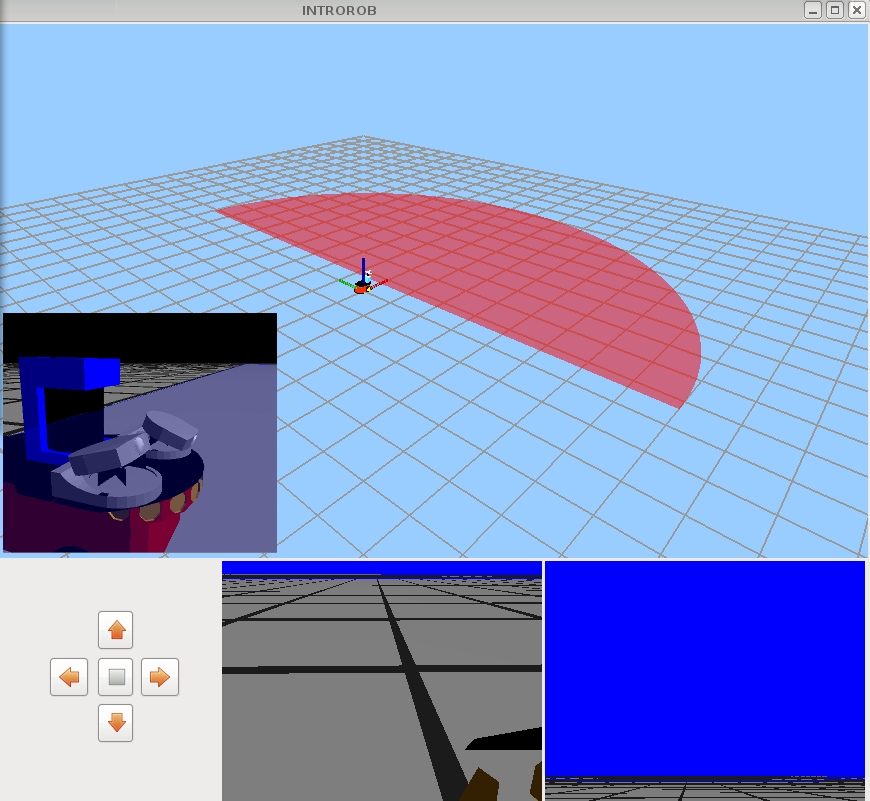
\includegraphics[width=8.5cm]{figs/introrob.jpg}
\caption{Introrob component interface.}
\label{fig:introrob}
\end{figure}

Having an integrated simulator is very important, so the students may quickly test their experiments without the need for a robot for every student. Such an environment is provided by The Player Project\footnote{http://playerstage.sourceforge.net/index.html} (see Section {subsec:gazeboserver}). This Open Source software is capable of simulating a population of robots, sensors and objects, but does so in a three-dimensional world.

\subsection{Robot navigation}

Obstacle avoidance is one of the key issues to successful applications of mobile robot systems. All mobile robots feature some kind of collision avoidance. It needs to steer the robot around the obstacle and proceed toward the original target.

We have implemented two famous navigation algorithms: VFF, as a obstacle avoidance or local path planning mechanism; and GPP, as a global path planner algorithm.

The Virtual Force Field (VFF) method is our earlier real-time obstacle avoidance method for our running robots. This technique allows for fast, continuous, and smooth motion of the controlled vehicle among unexpected obstacles, and does not require the vehicle to stop in front of obstacles.

On the other hand, when a trap-situation is flagged, the robot slows down (and may come to a complete halt),
while the VFF algorithm is temporarily suspended. The GPP algotithm is then invoked to plan a new path based on the available information in the gradient field that represents the optimal (lowest-cost) path to the goal at every point in the workspace (see Figure {fig:gppNav}).

\begin{figure}[h!]
  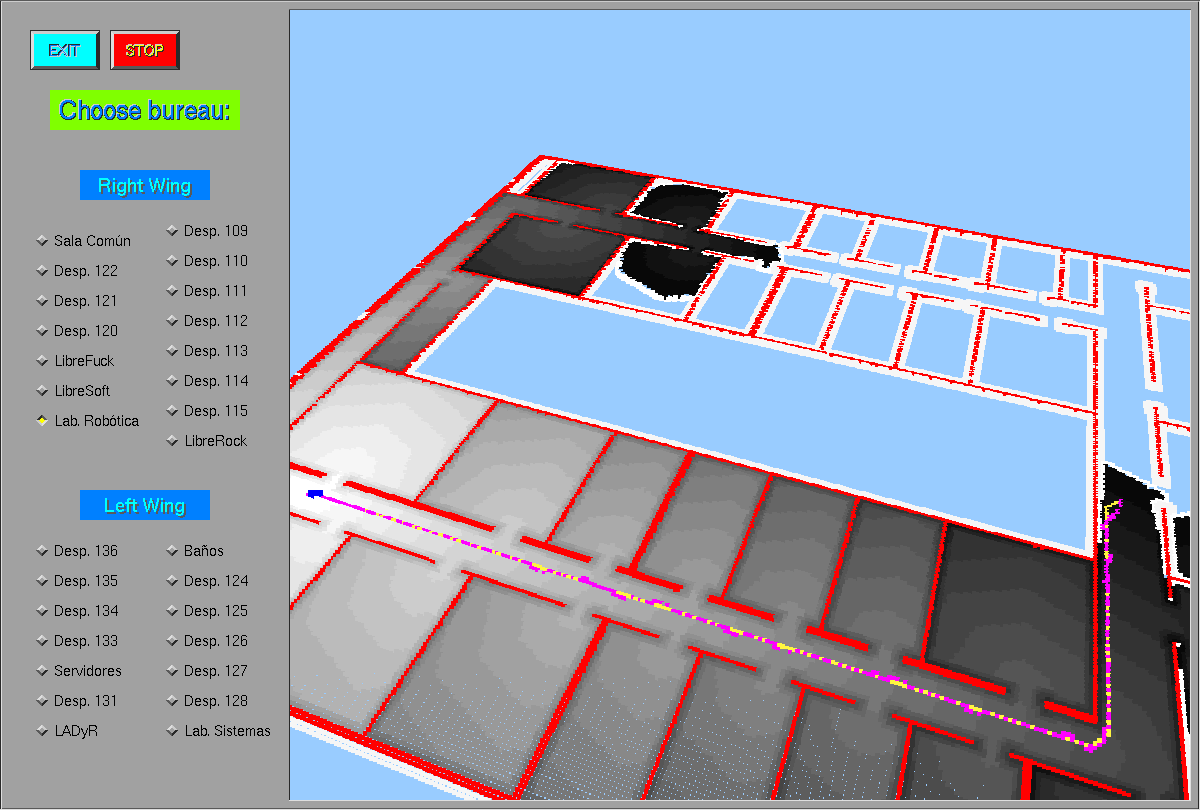
\includegraphics[width=8.5cm]{figs/gppNav.png}
\caption{Robot navigation using GPP and VFF algorithms.}
\label{fig:gppNav}
\end{figure}

Both techniques, VFF and GPP, have been implemented under Jderobot and extensively tested on Player-Stage and Gazebo simulators and on-board an ActivMedia Pioneer mobile robot, equipped with a ring of 24 ultrasonic sensors, and also using laser sensors, such as Hokuyo or Sick laser.

Follow person \cite{canas05d}.

\subsection{Evolutionary localization}

Self-localization is at the moment one of the most important challenges in robotics. Using robot sensors, such as cameras, laser sensors or ultrasonic sensors, our robot must be able to calculate its own localization inside an environment. Once the robot knows its position, it can adapt its behavior depending on where it is located. 
 
However, robot self-localization has proven to be one the most complex task on mobile robots, since they must face unknown situations, such as occlusions, or being located inside a dynamic environment.

With Jderobot, we have designed and implemented an evolutionary localization algorithm, a type of meta-heuristic optimization algorithm that is inspired by the biological evolution. In this kind of algorithms, candidate solutions evolve over time using genetic operators, such as mutation or crossover. 

The algorithm keeps several candidate solutions competing among each other in different positions. Thus, the evolutionary algorithm is able to handle several solutions at the same time, which is of great advantage when robots are located in symmetric environments.  

\subsection{MonoSLAM}

Monocular Simultaneous Localization And Mapping (MonoSLAM) is a type of localization first presented by Andrew J. Davison in 2003 (ref). MonoSLAM is able to construct a point-based map of the environment with a single camera, and localizates the camera inside this environment in real time.

We have developed our own MonoSLAM approach, based on Davison work, obtaining images from real cameras and simulators. We have implemented the point-based approach designed by Andrew Davison and afterwards we have designed our own implementations based on points and lines.

This type of localization is more accurate than classical localization methods and is very useful when robot odometry is not available or is not reliable. On the other hand, it is not able to handle occlusions and needs a faster frame rate.

% For two-column wide figures use
\begin{figure*}
% Use the relevant command to insert your figure file.
% For example, with the graphicx package use
  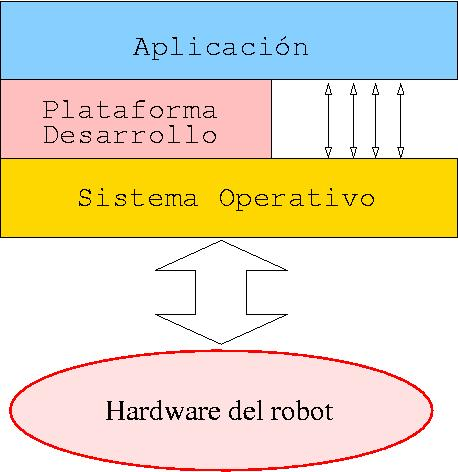
\includegraphics[width=7cm]{figs/programacion3.jpg}
% figure caption is below the figure
\caption{Please write your figure caption here}
\label{fig:2}       % Give a unique label
\end{figure*}


\subsection{Visual memory}

The goal of our visual memory is to do a visual tracking of the various basic objects in the scene surrounding the robot. It must detect new objects, track them updating its relative position to the robot and remove them from the memory once they have disappeared.

The first stage of the system is a 2D analysis, in which 2D segments in the current image are detected using the Solis algorithm \cite{solis09} (see Section \label{subsec:visionlib}). Then the system puts these objects in 3D space according to the \textit{ground-hypothesis}, assuming they all are flat on the floor, and stores them in memory maybe merging with already existing 3D segments. 

\begin{figure}[h!]
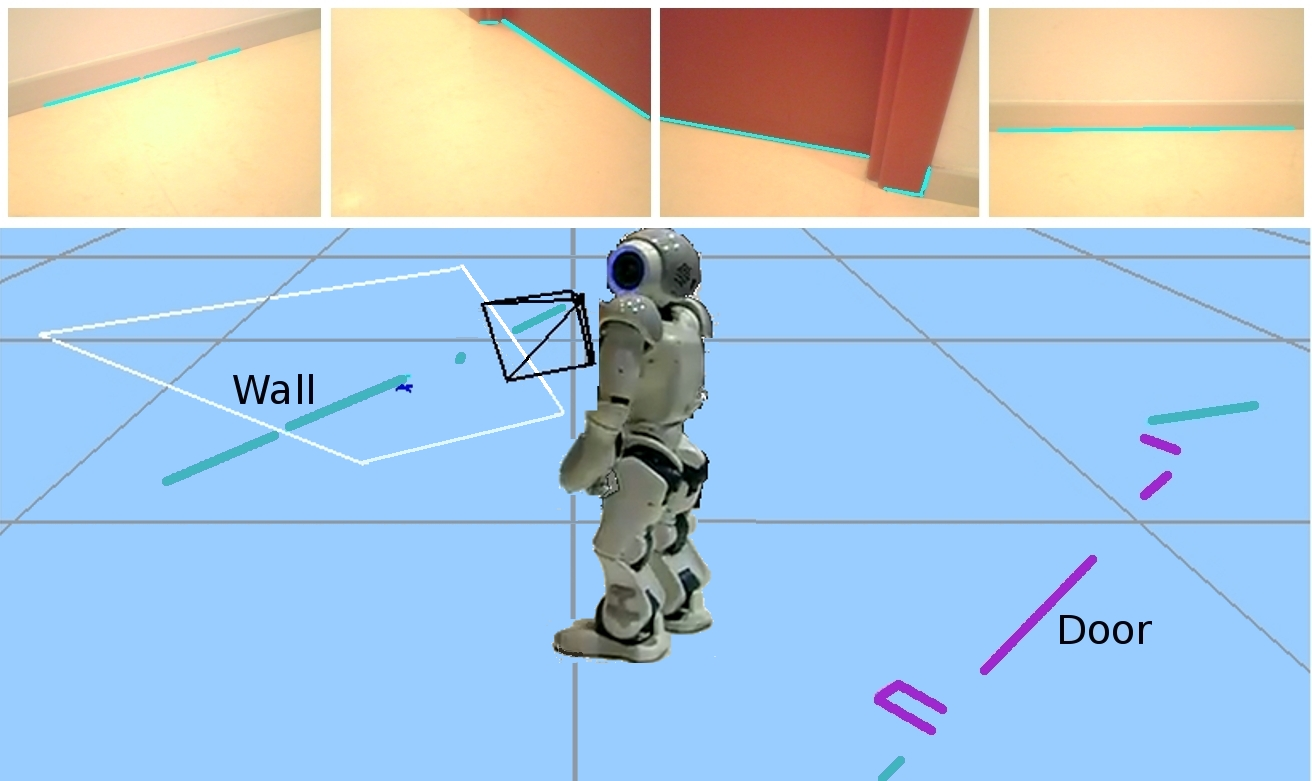
\includegraphics[width=8.5cm]{figs/experimentoReal.jpg}
\caption{Visual memory with 3D segments coming from four images of robot surroundings}
\label{fig:memory}
\end{figure}

Each 3D visible object already stored in memory is projected on the current image plane (using Progeo, see Section \label{subsec:progeo}. The system refutes/corroborates such predicted segments, comparing them with those extracted from current image. This comparison leads to three sets of segments. First, in case of matching the features of the stored 3D segment are updated taking into account the new observation. Second, if a segment is identified in the current image but does not match any prediction, the system creates a new one in 3D. Before inclusion in the 3D memory some post-processing is needed to avoid duplicates due to noise in the images, for instance comparing the relative position between segments, as well as its orientation and proximity. And third, for predicted segments not really observed in current image their quality goes down and eventually will be removed from memory.

\subsection{Surveillance}

\subsection{ElderCare}

\section{Jderobot as open-source project}

Jderobot project has a web page (jderobot.org) where the framework can be downloaded and its documentation accessed. The official manual is there in a MediaWiki. We prefer this web manual better than classic static documents, as the web manual update is agile and can be easily done by users themselves. We use a svn repository, trac for bug tracking, a blog and one mailing list for developers an users.

\subsection{Some history}

The Jderobot project started at 2003 in a PhD thesis, as the software implementation of a cognitive architecture to develop autonomous behaviors in robots \cite{canas02,canas05e}. It provided access to robot camera, encoders, sonar sensors and motors using sockets between some drivers and the (maybe remote) control application. The application was divided in \textit{schemas} that were implemented as concurrent threads in C language and organized as hierarchy. Its development was opened to a group of students. Several alternatives and expansions have been programmed since then \cite{canas07,canas07f}. 

A major revision was undergone in 2006. The design of schemas to be truly modular, they were programmed as dynamic libraries (plugins) which import and export symbols to other schemas. The XForms library for GUIs was replaced by GTK and OpenGL. In addition we started to use a common software repository and created a web page for the project. 

A second major revision was undergone in late 2010, leaving out the cognitive aspects and focusing in Jderobot simply as a software architecture for robot applications. The major design principles followed in this revision have been described in section \ref{sec:jderobot}. The current release, jderobot-5.0, is mainly based on this revision.

\subsection{Current release}
%current release and snapshot
Currently it has a total of 123.531 lines of source code, most of them in C and C++ language.

\begin{verbatim}
SLOC    Directory       SLOC-by-Language 
60707   src_components  cpp=32504,ansic=26370,
                        java=1355,xml=332,
                        sh=89,python=57
27509   src_interfaces  cpp=27509
23620   share           xml=23620
11354   src_libs        cpp=9979,ansic=1375
338     debian          sh=338
3       scripts         sh=3
\end{verbatim}

Totals grouped by language
\begin{verbatim}
cpp:          69992 (56.66%)
ansic:        27745 (22.46%)
xml:          23952 (19.39%)
java:          1355 (1.10%)
sh:             430 (0.35%)
python:          57 (0.05%)
\end{verbatim}

\subsection{Study of the Jderobot community}
% jderobot community, who is using Jderobot
The Jderobot community includes members of the Robotics Group at Universidad Rey Juan Carlos, the Universidad de Málaga, Universidad Carlos III and Politécnico Colombiano Jaime Isaza Cadavid. The last two have already developed new driver components for their specific robots: a worm type robot and an all-terrain wheeled one, respectively.
% It is not very large

One user profile is a regular student of robotics courses at URJC. They don't have too much time to learn all the issues and power behind Jderobot, they just want to use it as soon as possible focusing on their robotic practices. To hide most of the complexity of robot programming and let the alumni to focus on the key aspects of robot control (not in GUI neither in communication middleware, etc) the Introrob component was developed. They just have to embbed their control algorithm in it. In a four month course (2 hours/week) they are able to use Jderobot and program a robot behavior with a Finite State Machine, a local navigation algorithm and a reactive visual control technique. 

%\texttt{apt-get install jderobot}
In addition, some years ago only the Jderobot source code was delivered to students and its installation was painful for them, with different library dependences, etc. The installation of the Jderobot teaching environment was greatly simplified when we developed debian software packages for Gazebo and Jderobot.

A second user profile is a student from the URJC that use Jderobot for their Final Degree Project, Master or PhD thesis. They usually become developers and extend the framework in some area. This way, the developer team has frequently changed along years. Until 2006 these students typically took a snapshot of Jderobot software at the beginning of their project, extended it and maybe debugged for its own purposes. This was really a bad practice as improvements to the framework were not easily shared among students. Since 2006, with the Jderobot modular design and a single repository this was solved, forcing the students to always run their code with the latest Jderobot release, and debug only the official release if needed.

\begin{figure}
  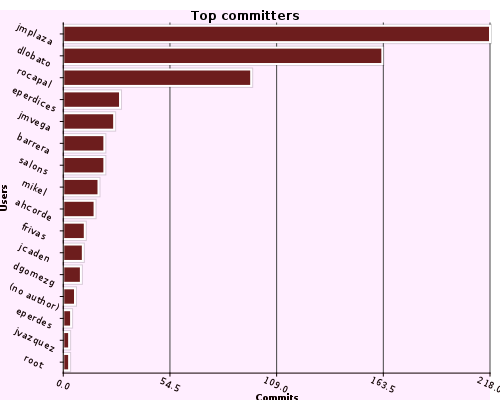
\includegraphics[width=7cm]{figs/svn_top-committers.png}
\caption{Top committers of Jderobot project}
\label{fig:svn-topcommiters}
\end{figure}

Some long term students have contributed continuously for several years, as can be seen at Figure \ref{fig:svn-topcommiters}. They have formed a stable developer core group of 4 or 5 people, all of them in a volunteer basis. In the last years, instead of having a reduced team of developers, we have opened the write access on Jderobot repository to relatively new users. Due to the large software size and the high rotation in the small developer team this has been very beneficial. The maintenance of the framework has already started to be more distributed.

\begin{figure}
  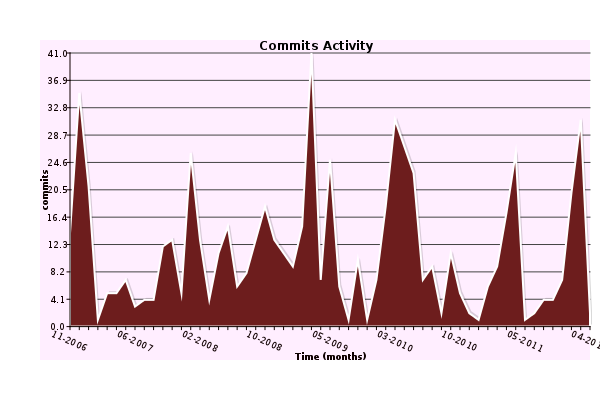
\includegraphics[width=7cm]{figs/svn_activity.png}
\caption{Activity of commits in the project}
\label{fig:svn-activity}
\end{figure}

Figure \ref{fig:svn-activity} shows the activity of software improvement as number of commits in the official repository. The high activity peaks are related with the release of a new Jderobot revision and its debugging period.

\section{Conclusions}

Modular design is good.

Open-source is advantageous: PCL, Gazebo, Opencv, OpenGL...

The use of svn and opening the development to several students was very beneficial.

True reuse in drivers. Not so (yet) in robot functionality.

Debian packages, easy the use of the platform in teaching, for newbie users that don't have time to fully understand the whole project.


\begin{acknowledgements}
This work has been supported by the project S2009/DPI-1559, RoboCity2030-II, from the Comunidad de Madrid and by the project 10/02567 from the Spanish Ministry of Science and Innovation. Authors want also to thank the contribution to Jderobot project to Alejandro Hernández, Maikel González and José Santos.
\end{acknowledgements}

% BibTeX users please use one of
\bibliographystyle{spbasic}      % basic style, author-year citations
%\bibliographystyle{spmpsci}      % mathematics and physical sciences
%\bibliographystyle{spphys}       % APS-like style for physics
\bibliography{bibliografia}   % name your BibTeX data base


\end{document}


